\chapter{Implémentation}
	\section{Introduction}
	
	Notre projet s'intègrent dans un projet de recherche scientifique. De ce fait, une implémentation efficace et optimisée de notre conception est nécessaire. Nous commencerons ce chapitre par présenter l'architecture existante et comment nous l'avons étendue avec nos deux moteurs tout en détaillant les différentes couches de la nouvelle architecture. Nous conclurons par présenter l'environnement de développement.
	
	
	\section{Architecture globale}
	
	L'architecture existante est une architecture en pipeline de 3-tiers. Elle se compose de trois couches logicielles que nous avons enrichie avec nos deux moteurs et la couche présentation. Nous les présenterons ci-dessous:
	
	\begin{enumerate}
	\item \textbf{La couche données ou persistance :} cette couche est responsable de la gestion des données en entrée et les fonctions d'accès et de stockage. Les données en entrées ainsi que les résultats de compression sont sous forme de fichiers.
	
	\item \textbf{La couche traitement :} c'est le noyau des moteur de compression de notre projet. Elle inclue tout les algorithmes de compression et de manipulation des graphes. 
	\item \textbf{La couche présentation :} cette couche permet de faciliter l'utilisation de notre solution à travers une interface simple et intuitive.
	\end{enumerate}
	
	
	
\begin{figure}[H]
	\centering
	\label{Img:archglob}
	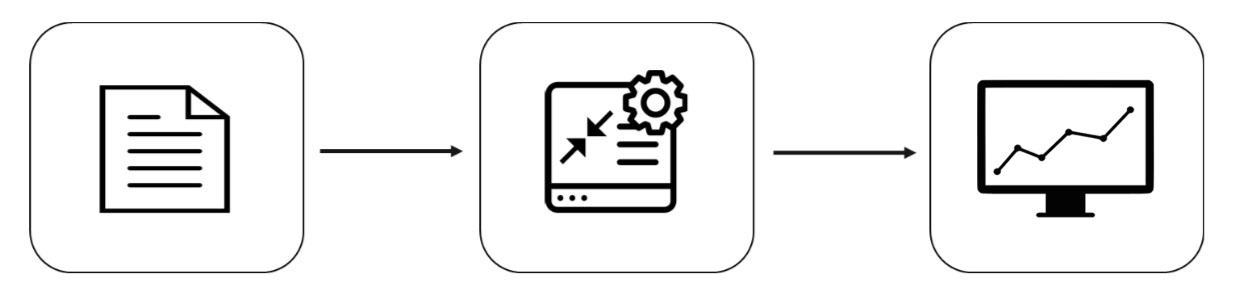
\includegraphics[scale=0.35]{ressources/image/ArchGlob.jpg}
	\caption{Architecture globale de la solution}

 \end{figure}
	
	
	
	\section{Données}
	Les données manipulées par notre solution sont tous sous format de fichiers textes. La structure de ses fichiers diffèrent selon le type de graphe en entrée. Comme nous l'avons déjà implicitement mentionnées, notre solution prend en charge les types de graphes suivant : graphe dynamique orienté, graphe statique orienté, graphe statique non orienté et finalement graphe statique étiqueté. Nous présenterons dans ce qui suit ses structures de fichiers:
	
	\begin{itemize}[label=$\bullet$]
	\item 1
	\item 2
	\item 3
	\item 4
	
	\end{itemize}
	
	
	
	\section{Traitement}
	\section{Présentation}
	
	La couche présentation est responsable de donner accès à toutes les fonctionnalités offertes par notre solution, entre autres le choix des paramètres pour différentes méthodes, ainsi que de visualiser les résultats. En plus du fichier de sortie, elle fournit les différentes mesures de performances. Elle offre ainsi aux chercheurs la possibilité de comparer les performances de différents méthodes sur un même graphe. Cette couche permet d'utiliser notre solution sans avoir recours à chaque fois au guide d'utilisation pour trouver les commandes d'exécution.
	
	\section{Environnement de développement}
		
		Le choix des outils de développement dans tout projet informatique est très important vue leur fort impact sur les performances du produit finale. Comme notre solution fait partie d'un projet de recherche, il faut aussi prendre en compte la flexibilité et la capacité de la solution à s'interfacer avec d'autre outils dans des systèmes qui peuvent être hétérogènes. 
		
		\subsection{Langage de Programmation}
		Nous avons adopté le langage de programmation avec lequel la    première version de notre solution a été développée: le C++. En effet, le langage C++ est un langage très performants pour les calculs lourds. Il permet d'avoir des exécutions très rapides, ce qui en fait un langage de choix pour les applications critiques qui ont besoin de performances. Il permet aussi d'avoir un code portable : un même code source peut être facilement transformé en exécutable sous Windows, Mac OS ou Linux. Un autre aspect du langage c++ est sa richesse de bibliothèques optimisées pour le traitement et le stockage des grands graphes en mémoire. 
		
		Nous avons choisi Visual Studio 2015 comme environnement de développement (IDE). Notre choix a été influencé par le fait que Visual Studio s'ouvre à toutes les tendances du moment et permet facilement de travailler en équipe sur le même projet.
		
		\newacronym{ide}{IDE}{Integrated Developement Environement} 
		\subsection{Bibliothèque Snap}
		
		\newacronym{snap}{SNAP}{Stanford Network Analysis Package}		
		Afin de faciliter la manipulation des graphes et d'améliorer les performances de notre solution, nous avons offert la possibilité d'exécuter les différents algorithmes de compression en utilisant une des plus performantes bibliothèque de manipulation de graphes en c++ : SNAP.
		\gls{snap} est une bibliothèque d'analyse et d'exploration de graphes à usage général qui s'adapte facilement à des graphes massives. Elle présente aussi l'avantage d'être  efficace et facilement extensible. Elle prend naturellement en charge les graphes riches avec des types de données complexes associés aux nœuds et aux arêtes. 
		
		\subsection{Bibliothèque Boost}
		

Boost est un ensemble de bibliothèques pour le langage de programmation C ++ qui prend en charge des tâches et des structures telles que l'algèbre linéaire, la génération de nombres pseudo-aléatoires, le multithreading, les expressions régulières et les tests unitaires. Elle contient plus de quatre vingt bibliothèques individuelles.

Nous l'avons utilisées dans notre projet pour l'implémentation des arbres $k^2$-trees. En effet, elle contient une implémentation des tableaux de bits en c++ qui donnent un temps d'exécution optimale parmi toutes les autres implémentations existantes \citep{pieterse2010performance}.  



		\subsection{Bibliothèque Qt }
	\section{Conclusion}
	
Durant ce chapitre, nous avons présenté notre implémentation où nous avons essayer d'utiliser différentes bibliothèques permettant d'avoir de meilleurs performances. L'indépendance des différentes couches de l'architecture existantes nous ont faciliter la tache d'implémentation. Nous avons ainsi essayer de respecter cette indépendance afin de faciliter tout autre contribution future dans le projet. 

Nous évaluerons dans le chapitre suivant les différentes méthodes de nos deux moteurs en vue de l'obtention d'une étude comparative plus objective et plus clair.